\chapter{Technical system overview}

\section{Function requirements}
This section specifies the requirements set for the functions mentioned in figure \ref{fig:funcarch}.
\subsection{Generate flow}
In the project plan, a literature overview is given on perfusion phantoms, for a variety of organs, but also on physiological factors: perfusion rates, blood pressures, rates of stenosis et cetera. The TFR-GF requirements are based on the estimates by \cite{uren1994relation}, summarised in appendix \ref{app:physoverview}, \cite{chiribiri2013normal}, \cite{ho2014dynamic}, summarised in appendix \ref{app:physoverview_ho}, and \cite{slart2015pres}.

\begin{table} [H]
\caption{Function requirements for function: Generate flow}
\label{tab:funcreq_tec}
This table specifies the requirements for the generated flow and pressure.
\begin{tabular}{l|p{120mm}|}
	\makecell[l]{\textbf{Requirement} \\  \textbf{number}} & \multicolumn{1}{c}{\textbf{Description}}\\
	\hline
	TFR-GF01 & A constant flow is to be generated, i.e. non-pulsatile. \\
	TFR-GF02 & Flow generators need to be interchangeable. \\
	TFR-GF03* & Minimum achievable upper limit of myocardial perfusion is 300 mL/min/100g. Stress perfusion typicially between 190-300 mL/min/100g. \\
	TFR-GF04* & Minimum achievable lower limit of myocardial perfusion is 60 mL/min/100g. Rest perfusion is typically between 60-95 mL/min/100g. \\
	TFR-GF05** & Minimum achievable upper limit of cardiac output is 8 L/min.\\
	TFR-GF06+ & Minimum arterial pressure is 56 mmHg. \\
	TFR-GF07+ & Maximum arterial pressure is  155 mmHg. \\
	TFR-GF08 & Flow generators are controlled via a flow feedback system. \\
	TFR-GF09 & Mean Arterial Pressure (MAP) \footnotemark is 89mmHg. Typical range is between 70 and 110mmHg.\\
	\cline{2-2}
\end{tabular}
\raggedright
\textit{* combined flow to myocardium, indicated by blue arrows in figure \ref{fig:sim_heart} }\\
\textit{** flow \textbf{not} entering the myocardium, indicated by red arrow in figure \ref{fig:sim_heart}} \\
\textit{+ based on the diastolic and systolic blood pressures, measured at dashed line P in figure \ref{fig:sim_heart}} \\
\end{table}

\footnotetext{Calculated as: $MAP \simeq DP + \sfrac{1}{3} (SP-DP)$}

\begin{figure}
\centering
\begin{minipage}{.5\textwidth}
  \centering
  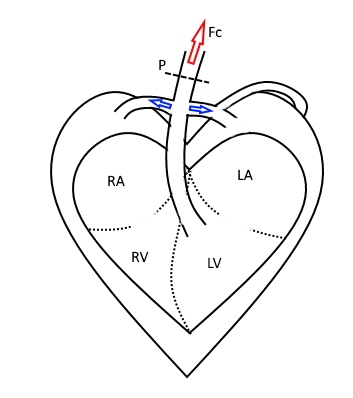
\includegraphics[width=0.7\linewidth]{./images/simplified_heart.png}
  \captionof{figure}{Simplified, schematic overview of the heart.}
  \label{fig:sim_heart}
\end{minipage}%
\begin{minipage}{.5\textwidth}
  \centering
  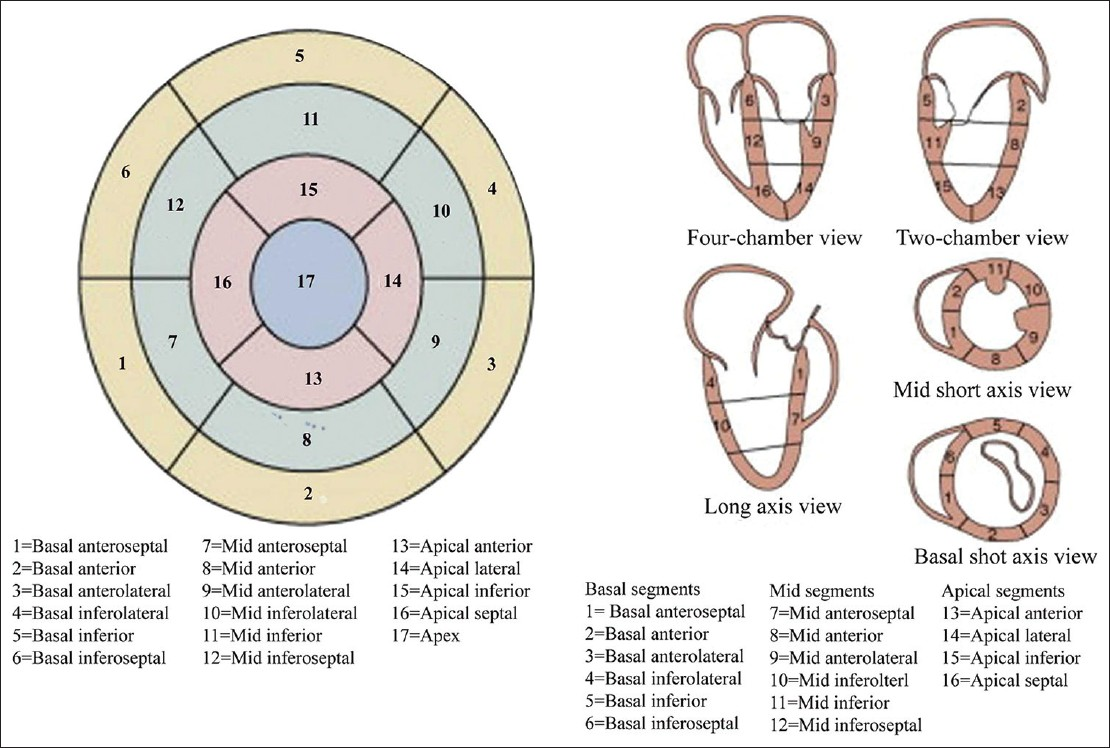
\includegraphics[width=0.95\linewidth]{./images/17_segment.jpg}
  \captionof{figure}{17-segment heart model}
  \label{fig:segment_heart}
\end{minipage}
\end{figure}

\subsection{Measuring flow and pressure}
\begin{table} [H]
\caption{Function requirements for function: Measure flow and pressure}
\label{tab:funcmeas}
This table specifies the requirements for the measuring of flow and pressure.
\begin{tabular}{l|p{120mm}|}
	\makecell[l]{\textbf{Requirement} \\  \textbf{number}} & \multicolumn{1}{c}{\textbf{Description}}\\
	\hline
	TFR-MFP01 & Flow measuring accuracy less than 5\%. \\
	TFR-MFP02 & Pressure measuring accuracy less than 5\%. \\
	TFR-MFP03 & Minimum absolute flow resolution of 1 mL/min. \\
	TFR-MFP04 & Minimum sampling rate of 100Hz. \\
	\cline{2-2}
\end{tabular}
\raggedright
\end{table}

\subsection{Simulate myocardial perfusion}
\begin{table} [H]
\caption{Function requirements for function: Simulate myocardial perfusion}
\label{tab:funcsim}
This table specifies the requirements specific for the phantom that simulates the myocardial perfusion.
\begin{tabular}{l|p{120mm}|}
	\makecell[l]{\textbf{Requirement} \\  \textbf{number}} & \multicolumn{1}{c}{\textbf{Description}}\\
	\hline
	\sout{TFR-SIM01} & \sout{An \ac{AIF} must be extractable from the left ventricle, as per software requirement.}\\
	TFR-SIM02 & Stenotic arteries are mimicked in a physiological way by physically narrowing (or increasing flow resistance) of certain arteries. \\
	TFR-SIM03 & Different stenotic severity, should be possible by, for example, variable flow resistors or interchanging components. \\
	TFR-SIM04 & The phantom must be compatible with D-SPECT protocol. \\
	\hspace{1.5cm} A) & Flow to the myocardium is supplied by the RCA, LAD, and LCx. \\
	\hspace{1.5cm} B) & Flow for each segment is supplied individually by branches of the RCA, LAD, and LCx, see figure \ref{fig:segment_supply}. \\
	\hspace{1.5cm} C) & Flow from each segment is measured separately such that they can be compared to the 17-segment model. \\
	\hspace{1.5cm} D) & An ROI for the AIF can be taken in the left atrium. Alternatively, the ROI for the AIF can be taken in the left ventricle. \\
	\hspace{1.5cm} \sout{E)} & \sout{An AIF can be taken from the left atrium.} \\
	\hspace{1.5cm} F) & The left ventricle's myocardium has a Vertical and Horizontal Longitudinal Axial (VLA/HLA) cross-sectional shape of a horseshoe. \\
	\hspace{1.5cm} G) & The left ventricle's myocardium has a Short Axial (SA) cross-sectional shape of a circle. \\
	TFR-SIM05* & Phantom's compartment model should match the currently practised protocol.\\
	\hspace{1.5cm} A) & The contrast agent specified as Technetium (\textsuperscript{99m}Tc) tetrofosmin, see section \ref{sec:inj_contrast}. \\
	\hspace{1.5cm} B) & The contrast agent is absorbed by the myocardium to approximately 1.2\% of administered activity in 5 minutes. \\
	\hspace{1.5cm} C) & Contrast accumulates in skeletal muscles, spleen, liver, and kidneys (potential interference). \\
	\cline{2-2}
\end{tabular}
\raggedright
\textit{* \url{https://pubchem.ncbi.nlm.nih.gov/compound/131704316\#section=Absorption-Distribution-and-Excretion}}
\end{table}

\begin{figure}
	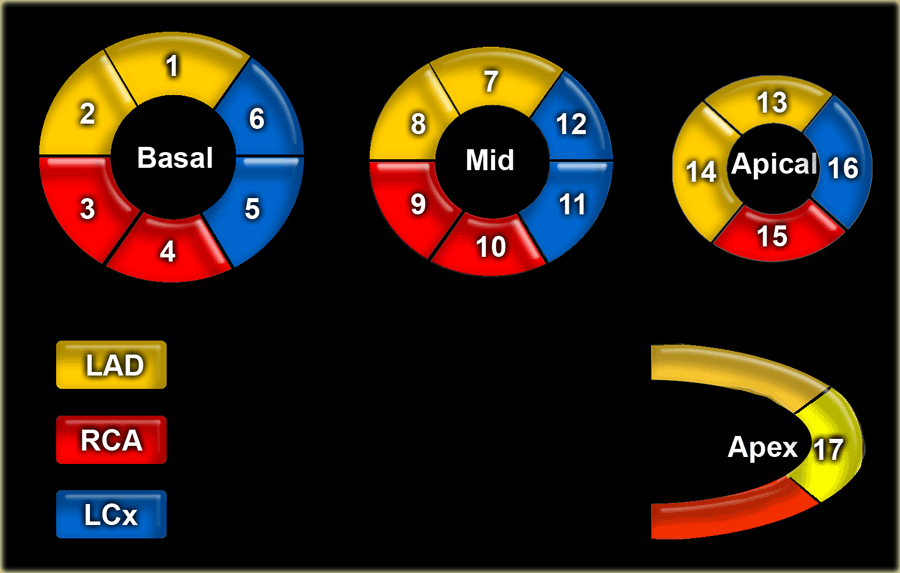
\includegraphics[width=0.5\linewidth]{./images/17_supply.png}
	\caption{Schematic representation of the supply to each segment.}
	\label{fig:segment_supply}
\end{figure}

\subsection{Inject contrast}
\label{sec:inj_contrast}
The injection protocol is not part of the development of the phantom. However, there are certain requirements to be monitored:
\begin{table} [H]
\caption{Contrast requirements}
\label{tab:injcon}
This table summarises the requirements on the contrast and contrast injection protocol.
\begin{tabular}{l|p{120mm}|}
	\makecell[l]{\textbf{Requirement} \\ \textbf{number}} & \multicolumn{1}{c}{\textbf{Description}}\\
	\hline
	TR-IC01 & Contrast volume is variable. \\
	TR-IC02 & Contrast injection is reproducible. \\
	TR-IC03 & Contrast protocol should match the currently practised protocol. \\
	\hspace{1.5cm} A) & Contrast agent is Technetium (\textsuperscript{99m}Tc) tetrofosmin. \\
	\hspace{1.5cm} B) & Contrast agent is injected, as bolus, via infusion pump. \\
	\hspace{1.5cm} C) & A pre-bolus is to be used of 37mBq, for proper placement of the heart in the scanner. \\
	\hspace{1.5cm} D) & A main bolus is to be used of 500mBq. \\
	\hspace{1.5cm} E) & A main bolus is to be used of 700mBq, for more hefty patients. \\
	TR-IC04 & Contrast concentration is variable. \\
	TR-IC05 & Contrast agent is variable. \\
	\cline{2-2}
\end{tabular}
\end{table}

\section{Physical requirements}
\rrow{Determine size of seating of D-SPECT}
\rrod{Determine weight limit of seating of D-SPECT}
\rrow{Must it be completely anatomical?}
\rrow{Adjust requirements if the phantom does not have to be anatomical.}
The following requirements state the physical aspects of the phantom and of the .
\begin{table} [H]
\caption{Physical requirements}
\label{tab:physrec}
This table summarises the physical requirements.
\begin{tabular}{l|p{120mm}|}
	\makecell[l]{\textbf{Requirement} \\ \textbf{number}} & \multicolumn{1}{c}{\textbf{Description}}\\
	\hline
	TR-PR01 & The phantom, and its set-up, must fit on the D-SPECT's chair. \\
	TR-PR02 & The phantom must be anatomically shaped. \\
	\hspace{1.5cm} A) & In correspondence with requirements TFR-SIM04 D). \\
	\hspace{1.5cm} B) & Four chambered phantom that correspond to left/right ventricle and left/right atrium. \\
	\hspace{1.5cm} C) & Myocardium surrounds heart chambers. \\
	\hspace{1.5cm} D) & Three coronary arteries, RCA, LAD and LCx, supply the myocardium. \\
	\hspace{1.5cm} E) & The coronary arteries run outside of the myocardium. \\
	TR-PR03 & The phantom must be placed inside a thorax phantom, QRM TRX-116, with maximum diameter of 100mm. \\
	TR-PR04 & Total weight, on patient chair, cannot exceed 171kg. \\
	TR-PR05 & The flow set-up must remain horizontal, to prevent additional flow resistance. \\
	TR-PR06* & The phantom must match the size of an average human heart, 12x8x6cm [LxWxD] \citep{openstax2013anatomy}. \\
	TR-PR07 & The phantom must resemble the weight of an average human heart, 250-300g (female) or 300-350g (male) \citep{openstax2013anatomy}. \\
	TR-PR08+ & The phantom's ventricles must match the volume of average human ventricles, between 40 and 180mL. \\
	TR-PR09+ & The phantom's atria must match the volume of average human atria, between 80 and 115mL. \\
	TR-PR10** & The phantom's ventricles must match the dimensions of an average human heart, between 60-90x30-50x60-90mm [LxWxD] \\
	TR-PR11 & The phantom cannot contain air bubbles. \\
	\cline{2-2}
\end{tabular}
\raggedright
\textit{*Length (L): longitudinal axis (apex-basal), width (W): transverse axis (septal - lateral), Depth (D):  transverse axis (anterior-inferior).} \\
\textit{**Length (L): longitudinal axis (apical-annular), width (W): transverse axis (septal-lateral (LV) or septal-medial (RV)), depth (D): transverse axis (apical-annular)} \\
\textit{+\cite{chiribiri2013perfusion} uses LA/RA of 105mL and LV/RV of 120mL.}
\end{table}

\section{Environmental requirements}
\rrot{Determine how much noise output it may have.}
\rrod{Determine the height of the chair of the D-SPECT}
In what environment is the system operating.
\begin{table} [H]
\caption{Environmental requirements}
\label{tab:envirreq}
This table summarises the environmental requirements, i.e. the restrictions set by the environment to the phantom.
\begin{tabular}{l|p{120mm}|}
	\makecell[l]{\textbf{Requirement} \\ \textbf{number}} & \multicolumn{1}{c}{\textbf{Description}}\\
	\hline
	TR-ER01* &  No high-density or "High-Z" material is to be used.\\ 
	TR-ER02 & The phantom's left and front side must remain free such that the D-SPECT camera image around it. \\ 
	TR-ER03** & Any part of the flow set-up and/or phantom, that does not fit directly on the patient chair, must remain horizontal with the remaining parts between 63 and 93cm. \\
	\cline{2-2}
\end{tabular}
\raggedright
\textit{* High-density and "High-Z" material, i.e. material with high atomic number, tend to block gamma radiation emitted by \ac{SPECT} tracers. Examples are Titanium (Ti), Chromium (Cr), Vanadium (V), Iron (Fe), or Lead (Pb); atom number \textgreater 22, Lead is 82.} \\
\textit{** The patient chair's seating is adjustable between 63 and 93cm.}
\end{table}

\section{External interfaces}
\begin{table} [H]
\caption{External interface requirements}
\label{tab:exint}
This table summarises the requirements for the external interface.
\begin{tabular}{l|p{120mm}|}
	\makecell[l]{\textbf{Requirement} \\ \textbf{number}} & \multicolumn{1}{c}{\textbf{Description}}\\
	\hline
	TR-EI01 &  Live plotting, at 10Hz, of system system flow and pressure.\\
	TR-EI02 & Ability to adjust the output of the flow generators. \\
	TR-EI03 & Serial communication between control/monitoring systems and external interface.\\
	\cline{2-2}
\end{tabular}
\end{table}

\section{System qualities}
\rrot{Specify pressure threshold.}
Define the quality of the system: such as reliability, availability, serviceability, security, scalability, maintainability.
\begin{table} [H]
\caption{System qualities}
\label{tab:sysqual}
This table summarises the system qualities.
\begin{tabular}{l|p{120mm}|}
	\makecell[l]{\textbf{Requirement} \\ \textbf{number}} & \multicolumn{1}{c}{\textbf{Description}}\\
	\hline
	TR-SQ01 & The flow set-up must perform an emergency shut down when the arterial pressure exceeds specified threshold. \\ 
	TR-SQ2 & The flow set-up must perform an emergency shut down when the flow cannot be controlled, i.e. erratic. \\
	\cline{2-2}
\end{tabular}
\end{table}

\section{Constraints and Assumptions}
Design constraints that have been imposed and assumptions that have been made by the requirements engineering team when gathering and analyzijng the requirements.

\begin{table}[H]
\caption{}
\label{tab:constassump}
This table summarises constraints placed on the design and assumptions made to yield the system requirements.
\begin{tabular}{l|p{120mm}|}
	\makecell[l]{\textbf{Reference} \\ \textbf{number}} & \multicolumn{1}{c}{\textbf{Description}}\\
	\hline
	TR-CA01 &  Cardiac artefacts, beating of the heart, is initially too complex. The phantom will be static. \\
	TR-CA02 & Breathing artefacts are not simulated in the phantom itself. A breathing thorax phantom can be used if available. \\
	TR-CA03 & Chest size, the amount of tissue between heart and scanner, is not simulated in the phantom itself. Thorax phantoms with modular rings are available to simulate tissue patients with varying BMIs. \\
	\cline{2-2}
\end{tabular}
\end{table}
